\uuid{h7Pm}
\exo7id{7061}
\titre{exo7 7061}
\auteur{megy}
\organisation{exo7}
\datecreate{2017-01-11}
\isIndication{true}
\isCorrection{true}
\chapitre{Géométrie affine dans le plan et dans l'espace}
\sousChapitre{Propriétés des triangles}
\module{Géométrie}
\niveau{L2}
\difficulte{}

\contenu{
\texte{
% collège
% orthocentre, triangle rectangle inscrit 
% cercle circonscrit, hauteurs
Soit $ABC$ un triangle. Le cercle $\mathcal C$ (resp. $\mathcal C'$) de diamètre $[BC]$  (resp. $[CA]$) coupe la droite $(CA)$ (resp. la droite $(BC)$) en $P$ (resp. $Q$). Les cercles $\mathcal C$  et $\mathcal C'$ se recoupent en un second point $R$. Montrer que $(CR)$, $(BP)$ et $(AQ)$ sont concourantes.

\begin{center}
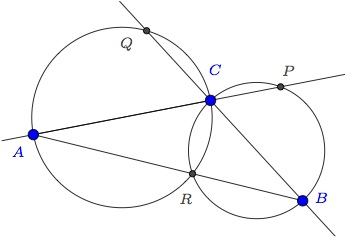
\includegraphics{../images/h7Pm-1}
\end{center}
}
\indication{Montrer que $(AB) \bot (RC)$.}
\reponse{
Un triangle dont un des côtés est un diamètre du cercle circonscrit est rectangle. On en déduit que les trois droites sont les hauteurs de $ABC$. Elles sont donc concourantes.

\begin{center}
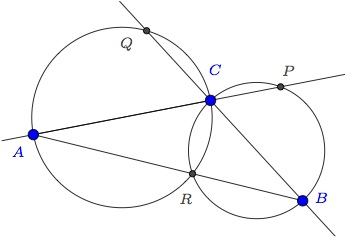
\includegraphics{../images/h7Pm-1}
\end{center}
}
}
